% TEMPLATE for Usenix papers, specifically to meet requirements of
%  USENIX '05
% originally a template for producing IEEE-format articles using LaTeX.
%   written by Matthew Ward, CS Department, Worcester Polytechnic Institute.
% adapted by David Beazley for his excellent SWIG paper in Proceedings,
%   Tcl 96
% turned into a smartass generic template by De Clarke, with thanks to
%   both the above pioneers
% use at your own risk.  Complaints to /dev/null.
% make it two column with no page numbering, default is 10 point

% Munged by Fred Douglis <douglis@research.att.com> 10/97 to separate
% the .sty file from the LaTeX source template, so that people can
% more easily include the .sty file into an existing document.  Also
% changed to more closely follow the style guidelines as represented
% by the Word sample file. 

% Note that since 2010, USENIX does not require endnotes. If you want
% foot of page notes, don't include the endnotes package in the 
% usepackage command, below.


% This version uses the latex2e styles, not the very ancient 2.09 stuff.
\documentclass[letterpaper,twocolumn,10pt]{article}
\usepackage{usenix,epsfig,endnotes,url, graphicx}
\graphicspath{{figures/}}
\begin{document}

%don't want date printed
\date{}

%make title bold and 14 pt font (Latex default is non-bold, 16 pt)
\title{\Large \bf Traffic Sign Classification}

\author{
	%for single author (just remove % characters)
	{\rm Colin Howes}\\
	University of Waterloo
} % end author

\maketitle

\thispagestyle{empty}


\subsection*{Abstract}

Efficient and accurate classification of traffic signs constitutes an interesting computer vision problem with a high degree of real-world relevance. Traffic sign recognition is necessary for the development of autonomous vehicles and driver assistance systems, which must be able to correctly detect and classify traffic signs in real-time under varying conditions. As such, traffic sign classification has enjoyed significant recent attention, and current techniques are able to meet or surpass human performance in publicly available data sets. Here, I compare successful approaches to traffic sign classification and present the performance of a simple traffic sign classifier based on a convolutional neural network.


\section{Introduction}

Traffic sign classification is a computer vision problem with a great deal of relevance to current advancements in autonomous vehicles and driver assistance systems. A viable traffic sign classifier must not only detect and categorize signs with a high degree of accuracy, it must perform efficiently, tolerate potentially noisy environments, and perform correctly in the presence of defects or variations in sign appearance \cite{stallkamp_german_2011, stallkamp_man_2012}. 

While many techniques have been applied to address the traffic sign classification problem, here I focus on a representative subset of state-of-the-art techniques that exhibit near-human performance in empirical testing: linear discriminant analysis, support vector machines, convolutional neural networks, and committees made up of multiple classifiers.

\section{Benchmarks}

The techniques discussed here were selected from high performing approaches entered into the German Traffic Sign Recognition Benchmark (GTSRB) competition, or developed and tested on this data set after the conclusion of the competition \cite{stallkamp_german_2011, stallkamp_man_2012}. This competition provides a high quality data set of traffic sign images split into training and test sets that can be used to design, validate, and compare approaches to traffic sign classification. The data set consists of 34799 training images and 12630 test images comprised of 43 classes. The data set is unbalanced, with class representation ranging from 0.5 \% and 5.5 \% of images \cite{stallkamp_german_2011}.

The German Traffic Sign Recognition Benchmark was originally formulated as a competition in two stages. Following the completion of the final stage, the GTSRB data set was made available online as a public benchmark to drive the development and empirical analysis of new classification algorithms. Additionally, human participants were also asked to classify images from the data set, correctly classifying 98.84 \% of examples on average \cite{stallkamp_german_2011, stallkamp_man_2012}. Here, I discuss the performance of classifiers entered at each stage of the competition, as well as other classifiers developed following the conclusion of the competition that provide an analysis based on the GTSRB data set.\footnote{It is worth noting that all of the published classifiers developed after 2012 that I have found as of this writing have provided an analysis using the GTSRB data set, so limiting discussion to approaches using this benchmark does not limit the scope of this paper.} 

\section{Comparison of Techniques}

\subsection{Features}

Traffic signs are designed to be easy for humans to detect and recognize quickly. In order to accomplish this, signs tend to be made up of distinct shapes, have high contrast lettering or pictograms, and strong colouration for high-importance sign classes (e.g.\ stop signs). The techniques discussed here make use of different feature sets to drive training and classification. 

While contrast and colour are fairly easy to define based on RBG and grey-scale pixel values, other features are more difficult to represent. In particular, histograms of oriented gradient (HOG) are commonly used by image classification algorithms as a means of determining shape and orientation information. Briefly, the orientation of pixel values across image subregions are computed and combined hierarchically to produce feature vectors representing geometric information about an image \cite{stallkamp_german_2011, stallkamp_man_2012}. A number of other features were preprocessed and made available along with the GTSRB data set, but they were not used in any of the classifiers compared here, so they are not discussed.


\subsection{Linear Discriminant Analysis}

Linear discriminant analysis (LDA) is a statistical method that can be used to find a linear combination of features characterizing a set of classes. Basic LDA can be used to construct a linear classifier separating two classes, but LDA classifiers can be combined to create higher dimensional classifiers, such as those needed for traffic sign recognition \cite{xanthopoulos2013linear}.

LDA gives fairly good results when applied to image classification problems, and is very fast both in training and classifying data \cite{hastie2001linear, mathias_traffic_2013}. LDA classifiers based on HOG features were used as a baseline model in the GTSRB competition, with the best implementation achieving a correct classification rate of 95.68 \%. While LDA is not as accurate as other methods, both training and classification time for the complete GTSRB data set are very low, on the order of seconds, making LDA very attractive for use with less powerful hardware in situations where real-time performance is required \cite{mathias_traffic_2013}.

\subsection{Support Vector Machines}

Support vector machines (SVMs) are binary linear classifiers designed to find the best separation between two classes based on a training data set. Like LDA implementations, SVMs can be used to produce non-linear and higher dimensional classifiers necessary for tasks such as traffic sign recognition \cite{mathias_traffic_2013}. SVM-based classifiers perform marginally worse on the GTSRB data set than LDA implementations, with the highest scoring solution correctly classifying 94.23 \% of examples in the training set \cite{mathias_traffic_2013}. Moreover, the time needed to train and test examples using SVMs is highly dependent on the features used, with high-performing implementations based on HOG features requiring upwards of 15 hours to train, though more efficient implementations require on the order of minutes to train and test on the complete GTSRB data set \cite{stallkamp_german_2011, mathias_traffic_2013}. 

Overall, SVMs seem to exist in a ``worst of both worlds'' between neural networks and LDA implementations, exhibiting comparatively low correct classification rates while also incurring the cost of time intensive training and classification. This makes current SVM-based traffic sign classifiers poorly suited for real-world applications, though given that SVM performance is highly dependent on the feature set, it is possible that creating an efficient and performant SVM sign classifier is simply a matter of selecting the right feature set.

\subsection{Convolutional Neural Networks}

Convolutional neural networks (CNNs) are multi-layer neural networks that consist of convolutional and pooling layers that feed forward into a classifier layer, which uses the inputs from previous stages to assign a probability distribution over a set of classes to a given example. CNNs are inspired by neurons in the visual cortex, where clusters of neurons process sensory data hierarchically, propagating signals in response to input patterns and allowing for fast, accurate recognition of visual stimuli. In CNNs, convolutional layers perform ``convolutions'' on inputs, such that each neuron in the layer responds to inputs for a specific region of input data, passing signals to layers further in the network. Pooling layers combine the output of clusters of neurons before sending an output to a neuron in the next layer. Finally, the output of the final stage is passed into a classifier, and a final output is ultimately used to assign a probability distribution to a given example \cite{ciresan_committee_2011, ciresan_multi-column_2012, sermanet_convolutional_2012, sermanet_traffic_2011}. 

One of the major advantages of CNN-based approaches is that images require little preprocessing, and the classifier does not make use of handcrafted features during training or classification. Rather, features are inferred at each stage of the classifier by the network, which learns a classification function from the training set over a series of training ``epochs'', making architectures easy to generalize across related problems \cite{sermanet_convolutional_2012, sermanet_traffic_2011, stallkamp_german_2011, stallkamp_man_2012}. 

Traffic sign classifiers based on CNNs perform well on the GTSRB data set, with the highest performing implementations reaching or exceeding human performance with the highest performing implementations  classifying between 98.31 \% and 99.17 \% of examples correctly. Unfortunately, the accuracy of CNNs comes at the cost of long training times, with training on the GTSRB data set taking on the order of hours and requiring access to powerful hardware \cite{sermanet_convolutional_2012, sermanet_traffic_2011, stallkamp_german_2011, stallkamp_man_2012}. 

CNNs are capable of providing highly accurate classification at the cost of a relatively large initial time investment needed to train the model. Additionally, high performance CNNs often rely on expensive hardware, making CNN implementations infeasible on low cost or lightweight embedded hardware.

\subsection{Committees}

The accuracy of classification algorithms can be improved considerably through the use of \emph{committees}, which are sets of classifiers that generate results that can then be combined to compensate for error due to misclassifications in individual classifiers. The highest performing classifiers entered into the GTSRB competition were comprised of committees based on convolutional neural networks \cite{ciresan_committee_2011, ciresan_multi-column_2012, stallkamp_german_2011, stallkamp_man_2012}. The original design proposed at the initial stage of the competition was built using a combination of CNNs and multi-layer perceptrons. This approached not only outperformed both MLPs and CNNs alone, but was the only classifier to outperform human participants. The authors refined the design to use only committees of CNNs, with the most advanced implementation reaching 99.46 \% accuracy on the GTSRB data set \cite{ciresan_committee_2011, ciresan_multi-column_2012}.

This \emph{multi-column deep neural network} (MCDNN) is fairly simple in its design, consisting of 25 CNNs arranged in ``columns'', where each column is an 9-layer CNN. Each column generates a prediction for a given example, and these predictions are averaged across all columns to produce a combined result \cite{ciresan_multi-column_2012}. Although these findings indicate that MCDNNs are highly accurate, training a large grouping of deep CNNs takes an exceptional amount of computing power, requiring 37 hours to train on 4 high-end GPUs, making this approach impractical for real-world applications even on advanced hardware \cite{ciresan_multi-column_2012}.

Committees have also been used to improve the performance of support vector machines by cascading SVM classifiers trained on HOG features. This technique has been shown to be fast enough to classify a constant steam of images at 20 frames/second at a 200 ms latency. However, although forming committees provides an improvement over poor-performing SVMs, this technique achieved only 89.2 \% accuracy on the GTSRB data set \cite{greenhalgh_real-time_2012}.

In general, committees are effective at improving performance above that of individual classifiers. However, in the case of highly accurate MCDNN implementations, this comes at a major computational cost, making the technique impractical for most real-world applications. Additionally, given the promising performance of committees of SVMs, using committees of lightweight classifiers for real-time classification may be in interesting avenue for future research.

\subsection{Discussion}

In general, methods based on convolutional neural networks have been shown to offer extremely high accuracy, matching or even exceeding human performance \cite{ciresan_committee_2011, ciresan_multi-column_2012, sermanet_convolutional_2012, sermanet_traffic_2011}. This high accuracy comes at the expense of both training and classification time, with large networks requiring days to train. Additionally, access to high-end hardware is necessary in order to achieve real-time classification with a trained model, making it difficult to implement high performant CNNs in embedded hardware that may need to support other computationally expensive functionality such as lane detection \cite{ciresan_committee_2011, ciresan_multi-column_2012, lane-detection}.

Linear discriminant analysis and support vector machines can offer a significant advantage in terms of efficiency over neural networks, but at the cost of some accuracy. Although high performing LDA and SVM based techniques boast roughly 95 \% accuracy, this may not be acceptable for real-world situations where recognizing and reacting to a sign is critical for passenger safety. Moreover, the designers of the GTSRB competition note that some of the human control participants found the interface used to gather human responses was uninituitive and difficult to use \cite{stallkamp_german_2011, stallkamp_man_2012}. As a result, human performance may have been artificially low due to testing conditions, while the nature of the constructed data set was likely advantageous to the classifiers since each test case has a well defined class with none of the ambiguity associated with real-world driving scenarios. Thus, implementations that fail to match human performance in an artificial environment are likely not good candidates for use in real autonomous vehicles or other safety-critical applications.

As hardware continues to become more powerful, computationally expensive classifiers based on committees of neural networks will likely become more attractive due to their robustness and accuracy. Indeed, advances in powerful, highly parallel embedded components, such as FPGA, are already seeing use in the automotive industry and in autonomous driving research \cite{fpga, fpga2}.

Finally, the emergence of ``standard'' benchmarks for traffic sign classification is something that bears consideration. The motivating idea behind benchmarks is that they give researchers and developers a way to assess how well a system performs. The consequence of this is that systems end up being tailored towards high performance on a benchmark rather than on the task they are designed to perform. In the context of machine learning, this could lead to overfitting, such that classifiers perform well on benchmarks but not on real-world examples.

One solution to this issue is to adopt many different benchmarks, and use classifiers that perform well on all of them. This is solution suits the traffic sign classification problem well, given that different regions have adopted different sets of traffic signs and classifiers need to be trained on data from every region where it is expected to be used. Indeed, a number of public data sets have been released since the GTSRB data set was made public, including the LISA (United States) and BelgiumTS (Belgium) data sets \cite{mathias_traffic_2013, mogelmose_vision-based_2012}. By benchmarking traffic sign classifiers on a diverse set of benchmarks, we may be able to both prevent overfitting and improve generalizability. 

\section{Methodology}

In order to validate previous results demonstrating the effectiveness of convolutional neural networks for traffic sign classification, I implemented a simple traffic sign classifier based on a convolutional neural network and evaluated it using the German Traffic Sign Detection Benchmark data set \cite{stallkamp_german_2011, stallkamp_man_2012}. All training and evaluation was done on a desktop computer running Ubuntu Linux 17.10 with a quad-core Intel Core i5-4690K processor, 16 GiB DDR3 memory, and a 4 GiB Nvidia GTX 970 graphics card. All implementation was done in Python 3.6.3 using Keras on top of TensorFlow.

\subsection{Architecture}

My approach was similar to the approaches outlined in \cite{sermanet_convolutional_2012, sermanet_traffic_2011}, though the architecture I present here used all colour channels and is purely feed-forward, with the classifier layer connecting only to the final convolutional layer. Similar models have shown high performance in previous replications, including \cite{keras_traffic} and \cite{tensorflow_traffic}, and the simplicity of this architecture makes it an attractive choice for experimentation.

The model is made up of three pairs of feed-forward convolutional layers separated by $2 \times 2$ max-pooling layers. Each of these pooling layers feeds into a dropout layer which drops $1/4^{th}$ of its inputs. The final set of convolutional, pooling, and dropout layers are flattened and passed into a classifier layer, which feeds into a softmax output layer that returns a probability distribution over the classes for a given input. The prediction for a given input is simply the maximum over this probability distribution.

\subsection{Training}

I trained the models over 200 epochs using the default batch size of 32 and a learning rate of 0.001. I used categorical cross-entropy as the loss function and stochastic gradient descent as the optimizer, which is suggested for multi-label classification problems \cite{lasagne_loss}. Training the model on the GTSRB data set using the hardware described above took a total of 52 minutes and 44 seconds.

\section{Results}

When training with only unaltered images provided in the GTSRB data set, my model had an accuracy of 95.77 \% on the test set, requiring a total of 1.98 seconds to classify all 34799 test examples, indicating that with powerful enough hardware the model could easily keep up with the framerate of any conventional camera (usually 24 frames/second). The accuracy of the model is reasonably high considering its simplicity and the lack of data set augmentation, though the accuracy is considerably lower than both human performance (98.84 \%) and the performance of other classifiers implemented using CNNs (98.31 \% - 99.17 \%) \cite{sermanet_convolutional_2012, sermanet_traffic_2011, stallkamp_german_2011, stallkamp_man_2012}. Figure 1 and Figure 2 show the accuracy and loss of the network over 200 training epochs when trained only on unaugmented images provided in the GTSRB data set.

\begin{figure}
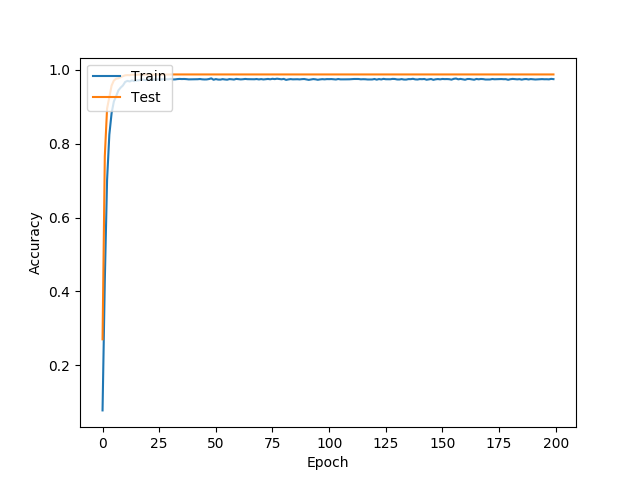
\includegraphics[width=3.25in]{accuracy}
\caption{Accuracy over 200 epochs on the base image set. Data for ``test'' instances are taken from performance on a validation set at the end of each epoch}
\end{figure}

\begin{figure}
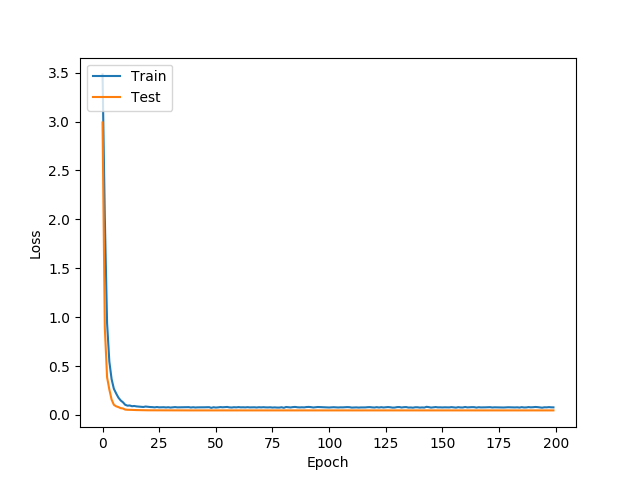
\includegraphics[width=3.25in]{loss}
\caption{Loss over 200 epochs on the base image set. Data for ``test'' instances are taken from performance on a validation set at the end of each epoch}
\end{figure}

In order to assess the benefit of augmenting the data set with simple transformations of training images, I trained the model again on the same architecture, randomly applying a Gaussian blur to $1/5^{th}$ of the training examples. I observed no improvement over the unaugmented data set, with the new model correctly classifying 95.38 \% of test images. Due to time limitations, it was not possible to experiment with other transformations, though I suspect that applying a random mix of transformations to generate the augmented data set would produce better results, since this technique has been used with considerable success in the past \cite{ciresan_committee_2011, sermanet_convolutional_2012}. Figure 3 and Figure 4 show the accuracy and loss of the network over 200 training epochs when trained the augmented data set.

Finally, I evaluated the effect of pairing convolutional layers before performing pooling to improve classification performance. The design of my architecture is based in part on a model similar to that used in \cite{sermanet_convolutional_2012}, though with the addition of paired convolutional layers prior to each pooling layer in place of a fully connected classifier \cite{keras_traffic}. I assessed the performance of my network without these additional layers and found that training time was reduced by roughly 40 \%, though the model was only able to correctly classify 91.19 \% of examples following training, suggesting that these additional layers are necessary in the absence of a fully connected network in which all layers feed into the classifier \cite{sermanet_convolutional_2012}.

\begin{figure}
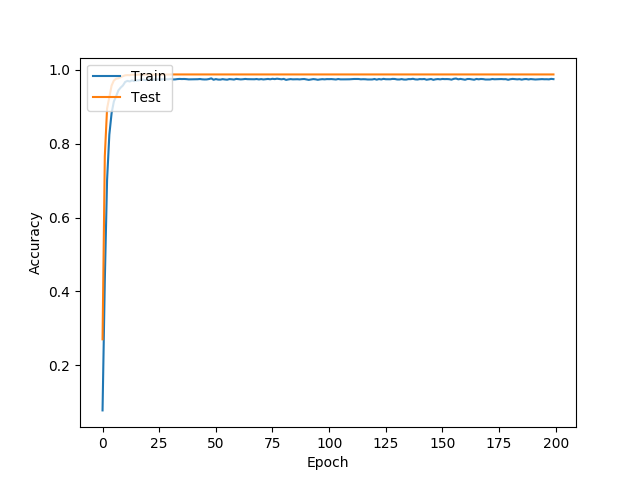
\includegraphics[width=3.25in]{accuracy}
\caption{Accuracy over 200 epochs using data augmentation. Data for ``test'' instances are taken from performance on a validation set at the end of each epoch}
\end{figure}

\begin{figure}
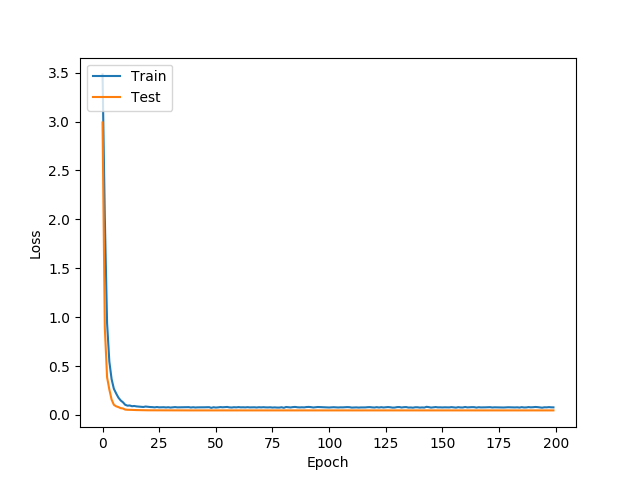
\includegraphics[width=3.25in]{loss}
\caption{Loss over 200 epochs using data augmentation. Data for ``test'' instances are taken from performance on a validation set at the end of each epoch}
\end{figure}


\section{Conclusions}

The results discussed above demonstrate that even a simple convolutional neural network can obtain reasonable speed and accuracy when trained with a high quality data set. Although I failed to demonstrate any benefit of data augmentation, the success of this technique in past work indicates that this is a failure in my relatively simplistic methodology rather than an issue with the technique itself \cite{ciresan_committee_2011, sermanet_convolutional_2012}. If I were to repeat this experiment again, I would add a more comprehensive set of transformations in computing the augmented data set. 

\section{Summary and Future Directions}

I presented an analysis and comparison of a set of traffic sign recognition techniques that performed well on a competition data set. In addition, I presented a simple implementation of a traffic sign classifier using a convolutional neural network and compared the effectiveness of this implementation with the performance of past techniques, though I failed to find any benefit in applying Gaussian blur to a random subset of training data in order to augment my data set.

Given the high accuracy of traffic sign classification techniques based on convolutional neural networks, future work should continue to improve the efficiency of these classifiers. Moreover, given the importance of real-time classification, future work investigating the use of neural networks for traffic sign classification should place more emphasis on efficiency. Future benchmarks may wish to take efficiency into account when considering the evaluation of techniques, perhaps by penalizing low throughput or high CPU/GPU usage.

Additionally, given the effectiveness of committees in improving accuracy beyond that of individual classifiers, future work should consider the use of committees of lightweight classifiers, such as implementations based on linear discriminant analysis, which provides relatively high accuracy given its low computational demands.

{\footnotesize \bibliographystyle{acm}
\bibliography{refs.bib}}

\end{document}
